\documentclass[conference]{IEEEtran}
\usepackage[english]{babel}
\usepackage{graphicx}
\usepackage[utf8]{inputenc}
%\usepackage[spanish]{babel}
\begin{document}

\title{Weather sensor fault detection in meteorological masts}

\author{\IEEEauthorblockN{Franco Piergallini Guida}
\IEEEauthorblockA{\textit{Universidad de Palermo}\\
Buenos Aires, Argentina \\
francopierguida@gmail.com}

\and
\IEEEauthorblockN{Maximo Iaconis}
\IEEEauthorblockA{\textit{Universidad de Palermo}\\
Buenos Aires, Argentina \\
iaconis@live.com.ar}

\and
\IEEEauthorblockN{Filippo Visco-Comandini}
\IEEEauthorblockA{\textit{Universidad de Palermo}\\
Buenos Aires, Argentina \\
fvisco@palermo.edu}
}


%\author{Franco Piergallini Guida, Maximo Iaconis, Filippo Visco-Comandini}
\maketitle

\begin{abstract}
Wind power has become the world's fastest growing renewable technology. The world-wide wind power installed capacity has exceeded 597 GW, and the new installations during the last three years was an average of 50 GW per year. A major issue with wind power system and with meteorological masts is the relatively high cost of operation and maintenance (OM). Wind turbines and sensor towers are hard-to-access structures, and they are often located in remote areas. That's why continuous monitoring of wind turbine health using automated failure detection algorithms can improve turbine reliability and reduce maintenance costs by detecting failures before they reach a catastrophic stage and by eliminating unnecessary scheduled maintenance.
Most of the wind turbines and meteorological masts have supervisory control and data acquisition (SCADA) system and it rapidly became the standard. SCADA data analysis has been used in other industries for accurate and timely detection, diagnostics and prognostics of failures and performance problems.
In the present work, mathematical methods are proposed for sensor fault detection for meteorological masts through the analysis of the SCADA data. The idea is to compare and analyze measurements coming from the various sensors located in the same tower and different heights. We used a number of measurements to develop anomaly detection algorithms and investigated classification techniques using manual check and model parameter tuning. 
These methods are tested on wind masts situated in Argentina.
\end{abstract}
\section{Introduction}
Renewable energy source is playing an important role in the global energy mix, as a mean of reducing the impact of energy production on climate change and wind power has become the fastest growing renewable technology. 
Wind energy is fundamentally used to produce electric energy. Wind turbines (WTs) are unmanned, remote power plants.  Efforts have been made to develop efficient and cost-effective condition monitoring techniques for wind turbines \cite{yang2014wind}. Unlike conventional power stations, WTs are exposed to highly variable and harsh weather conditions, including calm to severe winds, tropical heat, lightning, arctic cold, hail, and snow. Due to these external variations, WTs undergo constantly changing loads, which result in highly variable operational conditions that lead to intense mechanical stress \cite{ribrant2006thesis}. \\
Supervisory control and data acquisition (SCADA) is an application that collects data from a system and sends them to a central computer for monitoring and controlling. Current controlling monitor (CM) systems essentially provide the necessary sensor and capability of data capture required for monitoring.\\
In contrast to control engineering applications, the weather sensor fault detection has a few special features. Namely, the phenomenon itself, weather, can be non-linear and time-varying. The local fault detection model for the weather measurement can change drastically and disturbances can be very large. Fault diagnosis systems aims at detecting and locating degradation in the operation of sensors as early as possible. This way, maintenance operations can be performed in due time, and during time periods with low wind speed. Therefore, maintenance costs are reduced as the number of costly corrective maintenance actions decreases. Besides, the loss of production due to maintenance operations is minimized \cite{luo2014wind}.\\
The research for  fault detection and diagnostic techniques for wind turbines has been widely studying  \cite{tchakoua2014wind,wymore2015survey,lu2009review}. Some of the techniques involves
clustering algorithms and principal components analysis \cite{kim2011use}, artificial intelligence based framework \cite{wang2014scada}, performance evaluation and wake analysis \cite{astolfi2016mathematical}, machine learning algorithm \cite{kusiak2011prediction,schlechtingen2011comparative} and neuro fuzzy approach \cite{schlechtingen2012condition}.\\
Our research focus the fault diagnosis on meteorological masts,   
but the literature about these techniques is quite limited \cite{hasu2006weather} .\\
This paper proposes a methodology for fault diagnosis in sensor tower using a data-driven approach through the analysis of the SCADA data of two components. The anemometers and wind vanes measurements are analyzed with two different algorithms in order to develop anomaly detection techniques using manual check and model parameter tuning. Measurements comes from real-world wind turbines, that use same sensors.  \\
This paper is organized as following. In section \ref{sec:sensortower}, we describe the SCADA data coming from the two sensor tower components used in the algorithms, in section \ref{sec:failures} we show the different kind of failures that can happen in the sensor towers. In section \ref{sec:algorithms}, fault detection algorithms are presented. Results and discussion are in section \ref{sec:results} and the conclusion can be found in section \ref{sec:conclusion}.

\section{Meteorological mast components}\label{sec:sensortower}
Meteorological masts are towers made of steel where measuring components are installed. In this section we explain two components of sensor towers called anemometers and wind vanes and we describe how these components records their data through the SCADA system.
The sensor towers, are  lattice constructions consisting in three main beams shored up by smaller beams. The mast is a long slender construction, which gives an almost two-dimensional flow round a cross-section at certain height above the ground. 

\subsection{Components}
Meteorological masts usually have several measuring components, such as barometers, temperature sensors, but we focus in two of them.
\subsubsection{Anemometers}
An anemometer is a device for measuring wind speed. It consists in three horizontal arms where at each end an hemispherical cup is mounted. The air flow pushes the cups in any horizontal direction. Anemometers configuration involves offset, scale, boom orientation, units, and sensor height. Usually a sensor tower has on average six anemometers placed on different heights, and  anemometers are paired at each heights to have redundant measures \cite{clifton2014135}.
\subsubsection{Wind vane}
A wind vane is an instrument used for measure the winds direction. When mounted on an elevated shaft or spire, the vane rotates under the influence of the wind and the vane points into the wind. Wind direction is measured in degrees from true north \cite{sayigh2012comprehensive}.
\subsection{SCADA data}\label{subsec:scadaData}
SCADA systems are widely used for monitoring and control of Industrial Control System (ICS), including the emerging energy system, transportation systems, gas and water systems, and so on. The primary objective of a SCADA system is to control real-life physical equipment and devices, e.g., an energy system SCADA may be used for monitoring and controlling of the electrical plants \cite{ahmed2015investigation}. SCADA collects data from one or more distant facilities dispersed across a large geographic area. SCADA makes it unnecessary for an operator to be assigned to stay at or frequently visit remote locations when those are operating normally \cite{boyer2009scada}. \\
A functionality of SCADA system in a sensor tower is archiving the data coming from the data logger, the central computer instrument that records measurements from several sensors. Typically data are stored  on a cyclic basis: sometimes files are created based on file size, number of points of time period rate \cite{daneels1999scada}. In our case, the data logger archives time series measurements with a specific sampling rate set to be 10 minutes. \\
Through the paper, we will consider time series measurements $\{m_t^i\}$ for both wind directions and wind speed at time $t$ and on $i$-th positions of the sensor on the meteorological mast. For each time $t$, the data logger stores the minumum value, the maximum value, the standard deviation and the avergate of the measurements occured during the $t$-th 10 minutes interval.

\section{Failure in the sensor components}\label{sec:failures}
We are going to describe different existing
types of failures in sensor towers. In contrast to control engineering
applications, the weather sensor fault detection has a
few special features. %?Porque lo citamos??\cite{chandola2009anomaly}.


\subsection{Mechanical faults}
In the wind vane, mechanical failures correspond to a break in the head or tail of the instrument: usually these types of failures are produced by a lightning strike or hailstorms. They are reflected in the wind measurements only when the wind is going above or below a certain thresholds. Also, a mechanical faults could provoke a blockage of the wind vane and the results is a unrealistic fixed wind direction over a long period of time (See Figure \ref{fig:mechanicalfaults}).
\begin{figure}[h]
	\centering
	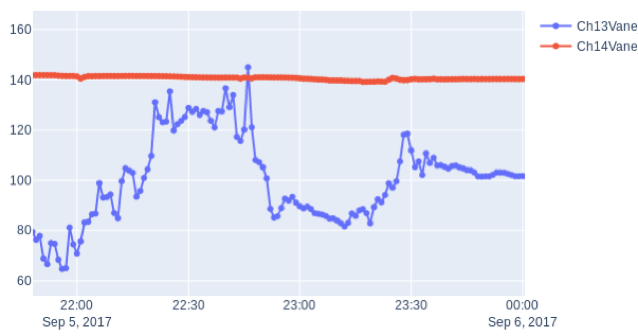
\includegraphics[width=\columnwidth]{Images/MechanicalFaults.png}
	\caption{Chanel Vane 14 is constant, because the wind vane is blocked. Chanel Vane 13 gives some realistic measures.}
	\label{fig:mechanicalfaults}
\end{figure}
In the anemometers, there is a large variety of mechanical faults and they are detectable in SCADA data. Lightning strikes or hailstorms could provoke a break on the anemometer's spoons, the wind speed measured by a broken anemometer could be both grater or lesser than the real value, depending on the breakage. Also, a blockage could occurs, preventing the rotation of the cups. They appear in certain specific wind conditions, for example when the wind speed is very slow.

\subsection{Connection faults}
Connection faults are due to a faulty connector between sensors, wires and the data logger. These faulty connectors make the measurements unstable in the sense that they are blocking the connections between sensors and the data logger (See Figure \ref{fig:connectionFaults}). The effect of the connection faults can interfere with the SCADA data in two possible way: either the faulty connections happens over a long period and hence they are reflected as intermittent values or it can happen between the sampling rate, making the standard deviation bigger than usual. \begin{figure}[h]
	\centering
	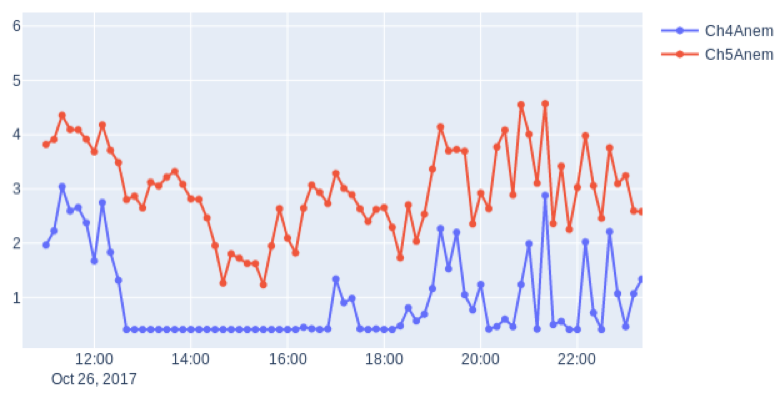
\includegraphics[width=\columnwidth]{Images/ConnectionFaults.png}
	\caption{The anemometer "Ch4" has some faulty connection wire and sometimes the wind speed drops to zero.}
	\label{fig:connectionFaults}
\end{figure}
\subsection{Calibration faults} 
Calibration faults are due to bad configuration of the data logger, it could be when it is initialized or when a sensor is replaced with another that has a totally different configuration and this is not updated on the data logger. Those faults are easily recognizable in the SCADA data, since their values have a constant offset compared to healthy sensors. In practice those type of faults change the measurement all along the scales (See Figure \ref{fig:calibrationFaults})
\begin{figure}[h]
	\centering
	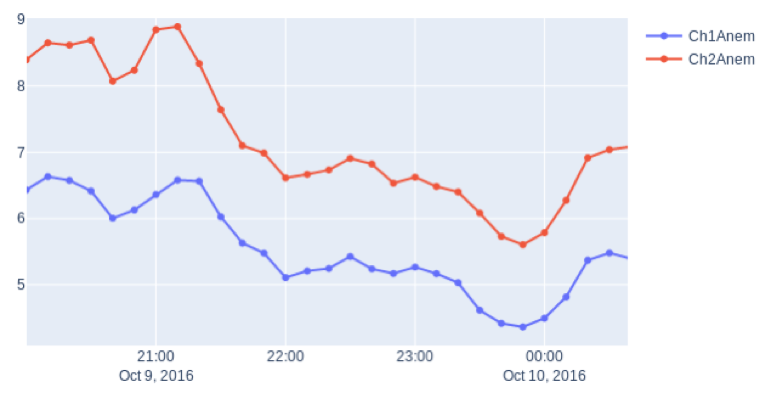
\includegraphics[width=\columnwidth]{Images/CalibrationFaults.png}
	\caption{In this case, the anemometer "Ch2Anem" was badly calibrated and it shows constant off with "Ch1Anem".}
	\label{fig:calibrationFaults}
\end{figure}
Sometimes both redundant sensor can have calibration failures.
Calibration is sometimes imposed by the data logger system, and rebooting the data logger may cause a failure in applying the correspondent calibration for each sensor for offset and slope.

\section{Algorithms}\label{sec:algorithms}
Anomalies are patterns in data that do not conform to a well defined notion of normal behavior. In this section we describe the algorithms used to detect anomalies. First, we need to define some auxiliary variables that allow us the possibility of flagging certains sensors. The flagging happens in various circumstances. Once variables are properly flagged, we show the logic to determine if a fault is detected.  
\subsection{Auxiliary variables}\label{subsec:computedvariables}
In the data logger, anemometers measures the wind speed and their units are expressed in \emph{m/s}. The wind direction is expressed as angle in degrees on a compass rose, where the origin is pointing to the North. In order to have a continuous values for the vanes' measurements, we consider their sinus values for these variables.
\subsubsection{Speed wind ratio}
The ratio is only computed for the anemometers type sensors. If $m_t^{i}$ represents the measurement at time $t$ on the $i$-th sensor, the ratio is defined as
\begin{equation}
R_{t}^{j,i} = \frac{m_{t}^{j}}{m_{t}^{i}},\qquad i \neq j,
\end{equation} 
for all possible sensor coupling. Paired anemometers produces reduntant measures because they are placed at the same  height in mast towers: in theory their ration should always be equal to 1.

\subsubsection{Speed wind Pearson correlations}
For the $i$-th sensor and for each time $t$, we consider the measurement vector with a time window $\omega$ as 
\begin{equation}
M^i_{t,\omega} = [m_{t-\omega}^i,m_{t-\omega+1}^i,\ldots,m_t^i]
\end{equation}
We compute the moving Pearson correlation depending on the time window $w$ between the $i$-th and the $j$-th sensors
\begin{equation}
C^{i,j}_{t,\omega}= \rho\left( \frac{M^i_{t,\omega}}{M^j_{t,\omega}}\right)
\end{equation}

\subsubsection{Wind direction difference}
The difference between vanes sinus values is computed as follow
\begin{equation}
D_{t}^{j,i} = {m_{t}^{j} - m_{t}^{i}},\qquad i \neq j 
\end{equation} 
for each couple of vanes.


\subsection{Flagging}\label{subsec:flagging}
At any time $t$, a variable is flagged if passes a specific threshold. Flagging a variable at a time $t$ means the correspondent sensor has an anomaly in the measurements.
These are the events that triggers the flag in particular time $t$
\begin{itemize}
\item $\|D_{t}^{j,i}\| \leq T_{vane}$
\item $\|C^{i,j}_{t,\omega}\| \leq T_{anem,C}$
\item $\|R_{t}^{j,i}\| \leq T_{anem,R}$
\item $s_t^i>T_{wind}$
\end{itemize}
where $T_{vane}$ is the threshold for vanes,  $T_{anem,C}$ is the correlation threshold for anemometers,  $ T_{anem,R}$ is the ratio threshold for anemometers,  and  $T_{wind}$ is the maxim wind speed threshold anemoters.\\ 
The last condition is fail condition for the anemeter. The average speed has certain limit $T_{wind}$: above this limit, the wind speed is not realistic and hence the sensor is faulty. In \cite{}, the speed wind threshold is set to $70$ \emph{m/s}.

\subsection{Fault detection}\label{subsec:faultdetection}

We consider that a sensor has a failure when the following conditions are verified for anemometers and wind vanes.
\subsubsection{Anemometer}
The $i$-th anemometer  detected as an anomaly if the following conditions are verified:
\begin{itemize}
	\item At least two measurements between $R_{t}^{j,i}$ and $C_{t}^{j,i}$ are flagged for $i \neq j$.
	\item At least one of the previous flag must belong to a reduntant sensor.
\end{itemize}

\subsubsection{Wind vane}
A wind vane is considered a faulty wind vane  only when 
\begin{itemize}
	\item At least one of $D_t^{i,j}$ is flagged.
\end{itemize}

\section{Results and discussion}\label{sec:results}
We tested our algorithms to two different real world datasets. Both of them are measurements coming from mast towers  for the period of 12 months located in Argentina and Mexico. Maintenance operations as well as any detected failures or sensor replacements are unknown.

The fault detection process is still a working in progress, and the detected faults were visually checked. Through the entire process, we were able to identify several realistic possible faults and we used them benchmarks to tunes various parameters.

With this process, we tuned the thresholds for vanes and anemometers ($T_{vane}$,$T_{anem,C}$,$T_{anem,R}$) and the correlation time window ($\omega$). We performed the algorithm for several ranges of values of the parameters and compare it with the realistic faults on data sets, in order to obtain the combination that has the best sensibility for detect real faults. (See Fig.\ref{fig:parametersAnalysis}).

\begin{figure}[h]
	\centering
	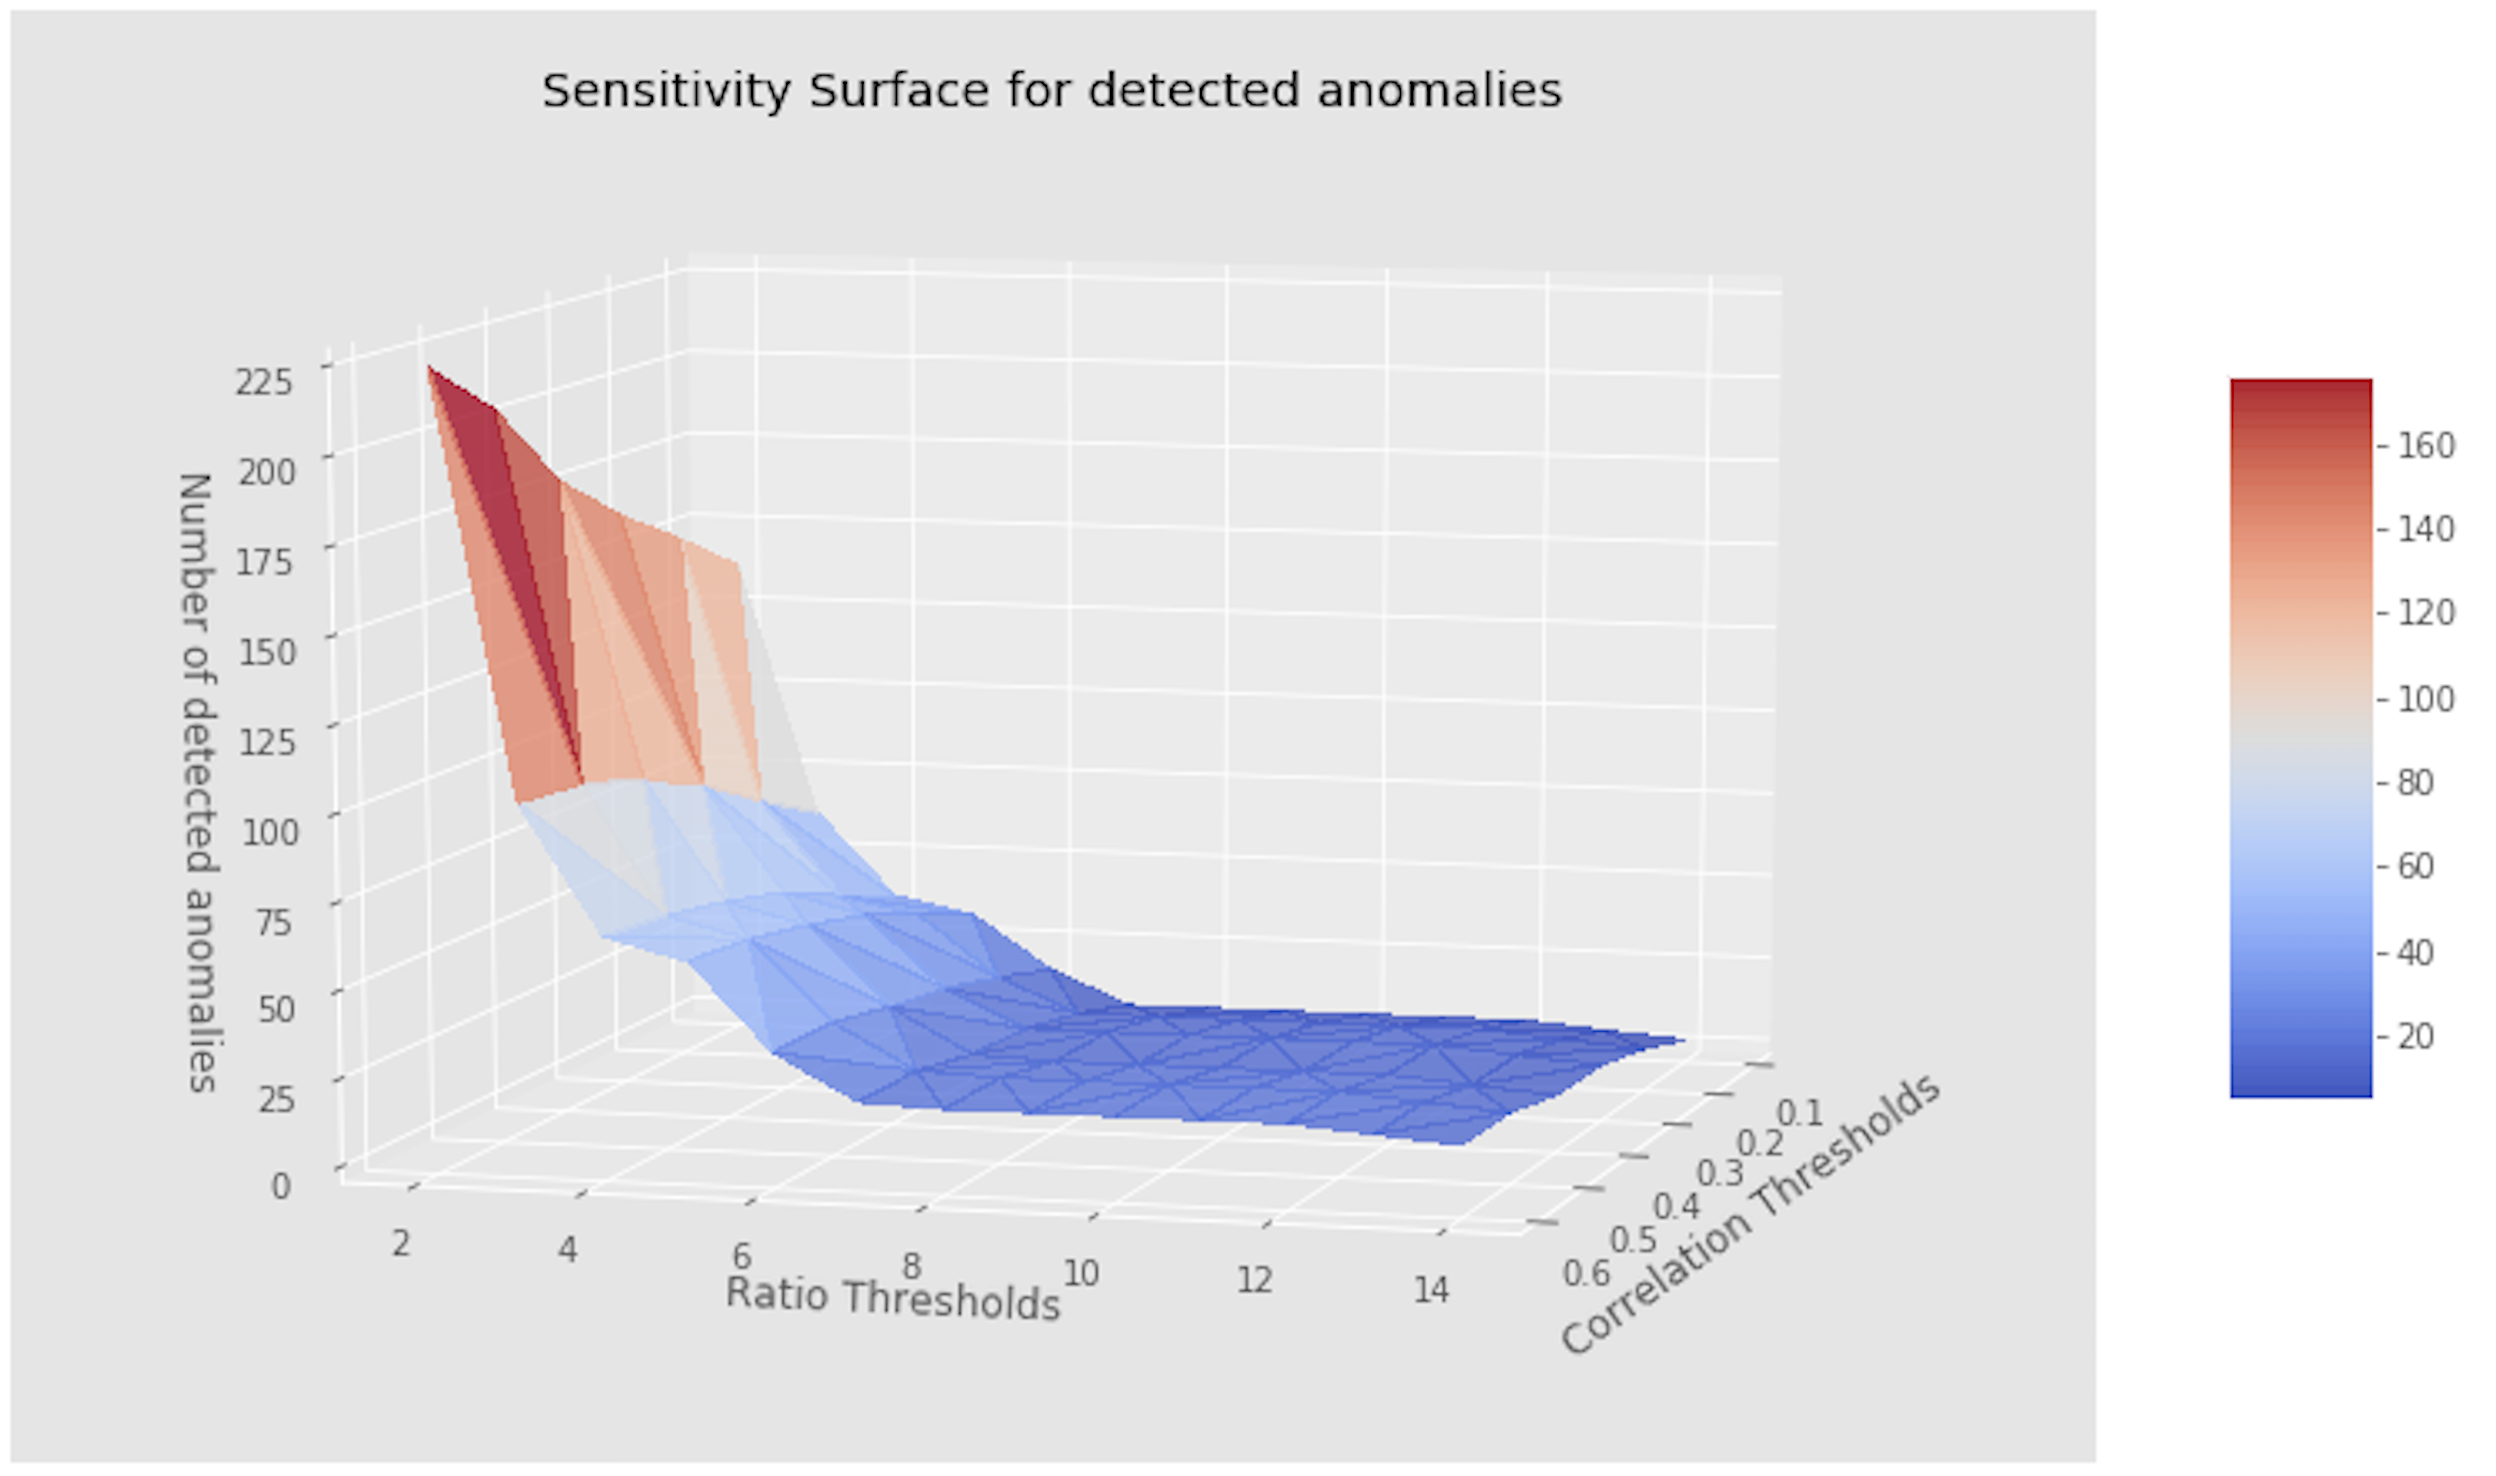
\includegraphics[width=\columnwidth]{Images/SensitivityAnalysis2.png}
	\caption{Parameters sensitivity analysis}
	\label{fig:parametersAnalysis}
\end{figure}

We concluded that the best choice for this parameters is given in the Table \ref{table:parameterChoice}.
\begin{table}[h]
\begin{center}
	\begin{tabular}{ |l|l| } 
	 \hline
	 Parameter & Values  \\ 
	 \hline
	 $T_{vane}$ & 0.1\\
	 $T_{anem,C}$ &0.5\\
	 $T_{anem,R}$ & 10 \\ 
	 $\omega$ & 3 \\
	 \hline
	\end{tabular}
\caption{Parameters values}
\label{table:parameterChoice}
\end{center}
\end{table}

Despite the promising results, our algorithm still need to be tested in a real world dataset in which the fault types and their locations are known.

\section{Conclusion}\label{sec:conclusion}

In the industry 4.0, the application of fault detection and prediction algorithms is crucial. In this context, we offered a solution to an real industrial problem. A methodology to predict faults using data provided by SCADA systems and fault files was presented. 

This work bring an initial research advancement for similary sensor analysis applied to wind turbines. Despite the fact this algorithm is still in a validation stage, once its reliability is confirmed, it can be applied to other sensor systems. The preseny work is a work in progress with the goal to become an effective fault detection system.
As future work, it si worth consider the prediction of the fault in sensors before they becomes blockers.

\bibliographystyle{ieeetr}
\bibliography{BibliografiaAERO.bib}

\end{document}


